\graphicspath{{./fig_Implement/}}



%%
\section{内部境界条件の実装のしくみ}

%
\subsection{BC Index}
計算空間の各セルおよびセルの各フェイスへの境界条件処理は,機能性と計算効率の点で注意深く実装すべき部分である.
空間スキームのカーネル部分と比べて,条件分岐などが多くベクトル化,SIMD化が利きにくいため,計算量を最小化する工夫が必要となる.
境界条件の空間的存在範囲は局所的な傾向であり,その計算は並列処理時のロードバランスを崩す要因なので,この点にも気をつける必要がある.
CBCの実装方針として,以下のポリシを基本とする.

\begin{enumerate}
\item 局所的な処理\\
境界条件の存在範囲を探索する領域を最小化するため,BV情報を利用する.
\item 演算量を最小化\\
前処理可能な部分は,保存メモリ量も少なくするようにして保持する.
\item 2パス計算\\
通常の空間演算処理を行い,境界処理が必要な部分だけ計算し,修正量を加える.
\item 高性能計算\\
通常の空間演算処理においても,計算空間内の任意部分に現れる固体壁面の処理を効率よく行う工夫が必要になる.
また,反復計算において,係数行列のロードコストを削減することも高速計算に必要になる.
\end{enumerate}


CBCソルバでは,様々な境界条件の情報を纏めて管理し,計算時に境界条件を効率的に実装するため,\textbf{図\ref{fig:BCIndexDP}}および\textbf{図\ref{fig:BCIndexVH}}に示すBC Index,CompoList クラス,MaterialList クラスを利用する.
BC Indexは,計算処理に必要なフラグ情報を4バイトのビットフィールドに機能を持たせたフラグをコンパクトに割り当て,領域空間における境界条件の設定のために利用する.
CompoList クラスは境界条件の種類やパラメータなどの情報,MaterialList クラスはセル属性を保持する.

\begin{figure}[htbp]
\begin{center}
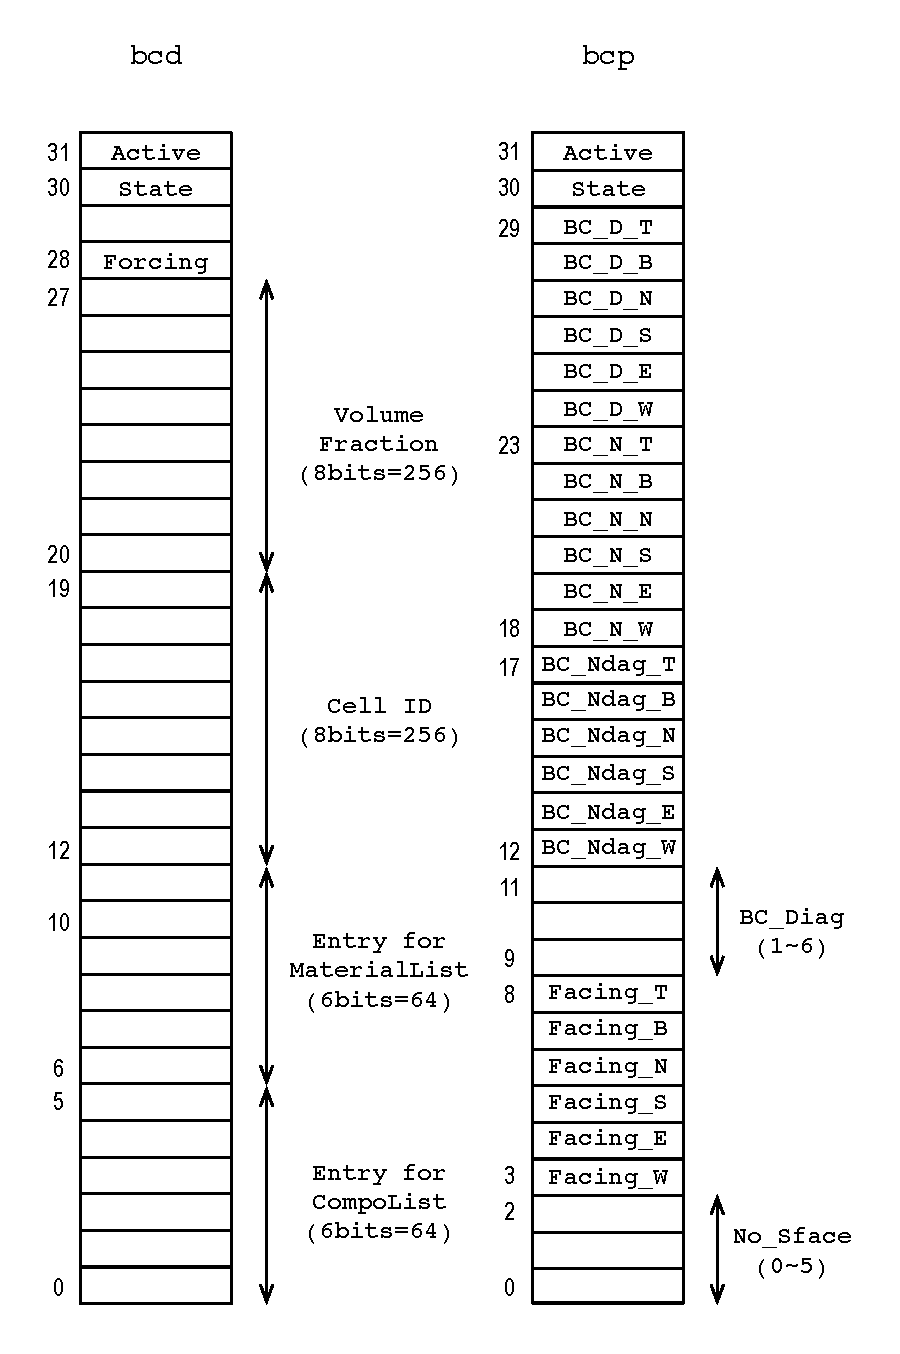
\includegraphics[height=11cm,clip]{BCindexDP.eps}
\end{center}
\caption{境界条件実装に用いるBC Index. bcd[]は共通要素,bcp[]は圧力計算に用いる.}
\label{fig:BCIndexDP}
\end{figure}

\begin{figure}[htbp]
\begin{center}
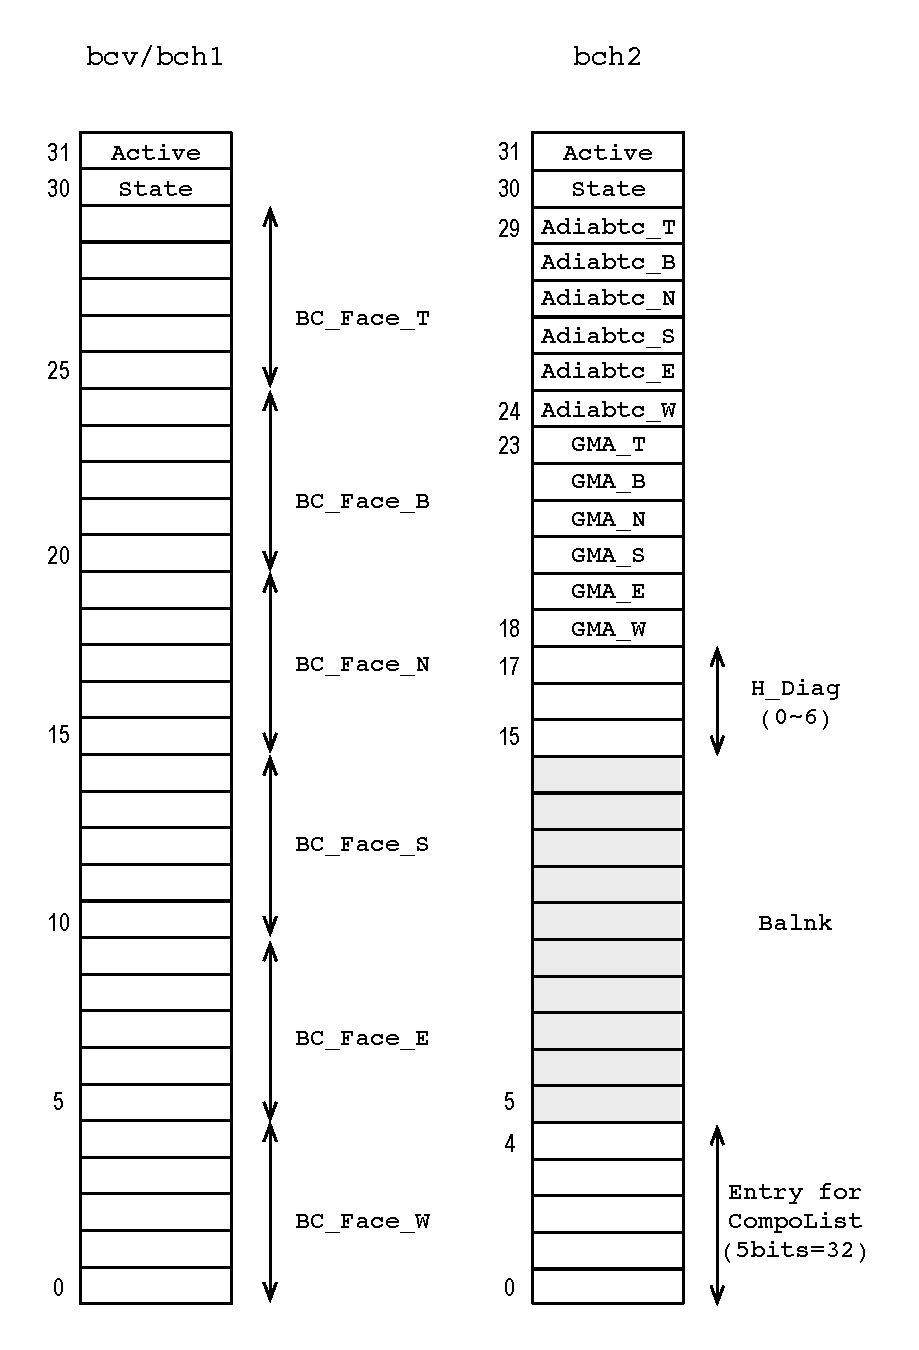
\includegraphics[height=11cm,clip]{BCindexVH.eps}
\end{center}
\caption{境界条件実装に用いるBC Index. bcv[]は速度計算,bch1, bch2[]は温度計算に用いる.}
\label{fig:BCIndexVH}
\end{figure}

bcd[]は計算空間を構成する各セルに対して割り当てられた配列で,\textbf{表\ref{tbl:Flags in bcd}}に示すように,共通的に利用する情報を保持する.
ComponentおよびMaterialは,それぞれ,CompoListとMaterialListクラスオブジェクト配列のエントリを格納する領域である.bh2[]でもCompoListへのエントリをエンコードするが,bcd[[]は全てのコンポーネントを保持する.一方,bh2[]では熱境界条件に必要なコンポーネントのみ保持する.
Cell IDはセルに割り当てられているIDを保持する.このIDはユーザが作成するボクセルモデルにより指定される.
Volume Fractionはセル内における流体の体積占有率を$0\sim255$の値で量子化した値を保持する.
Forcingは?.
Stateはセルの状態を指定するフラグで,排他的である.
Activeは対象セルが計算に有効かどうかを指定し,Kind\_of\_Solverの指定するモードにより異なる.

\begin{table}[htdp]
\caption{BC Index bcd[] に割り当てるビットフラグ(4バイト幅)}
\begin{center}
\small
\begin{tabular}{clll} \toprule
Bit & Flag & Property & Explanation\\ \midrule
31 & Active & 0-Invalid / 1-Valid & 対象セルが計算に有効かどうかを指定するフラグ\\
30 & State  & 0-Solid / 1-Fluid & セルの状態を指定するフラグ(排他的)\\
28 & Forcing & & \\
20$\sim$27 & Volume Fraction & 0-255 & 8bitで量子化された体積率[0,1]\\
12$\sim$19 & Cell ID & 1-255 & 8bit幅の正数\\
6$\sim$11 & Material & 1-63 & MaterialList[]へのエントリ(6bit幅)\\
0$\sim$5 & Component & 1-63 & CompoList[]へのエントリ(6bit幅)\\ \bottomrule
\end{tabular}
\end{center}
\label{tbl:Flags in bcd}
\end{table}

bcp[]は\textbf{表\ref{tbl:Flags in bcp}}に示すように,基本的に圧力計算に必要な情報を保持している.
No\_Sfaceは粘性項の修正に利用するための係数で実験的な実装である.
Facing\_?は,壁法則の計算などに利用するための情報で各セル方向に壁面があるかないかを示す.
BC\_Ndag\_?は反復計算時に利用する行列の対角要素の係数である.
BC\_Ndag\_?は同じく非対角要素の係数である.
BC\_N\_?とBC\_D\_?はぞれぞれ,Neumann条件とDirichlet条件のフラグであり,両者は同時に0ではありえない.

\begin{table}[htdp]
\caption{BC Index bcp[] に割り当てるビットフラグ(4バイト幅)}
\begin{center}
\small
\begin{tabular}{clll} \toprule
Bit & Flag & Property & Explanation\\ \midrule
31 & Active & 0-Invalid / 1-Valid & 対象セルが計算に有効かどうかを指定するフラグ\\
30 & State  & 0-Solid / 1-Fluid & セルの状態を指定するフラグ(排他的)\\
24$\sim$29 & BC\_D\_? & 0-Dirichlet / 1-Non Dirichlet(Default) & 各方向のセルフェイスのDirichlet境界フラグ\\
18$\sim$23 & BC\_N\_? & 0-Neumann / 1-Non Neumann(Default) & 各方向のセルフェイスのNeumann境界フラグ\\
12$\sim$17 & BC\_Ndag\_? & 0-境界条件あり / 1-境界条件なし & 各セルフェイス方向の係数\\
9$\sim$11 & BC\_Diag & [1-6] & 対角要素の係数\\
3$\sim$8 & Facing\_? & 0-壁面なし / 1-壁面あり & 各セルフェイス方向の壁面の有無(wall location)\\
0$\sim$2 & No\_Sface & [0-5] & セルの壁面の面数\\ \bottomrule
\end{tabular}
\end{center}
\label{tbl:Flags in bcp}
\end{table}

\textbf{表\ref{tbl:Flags in bcv}}に示すbcv[]は速度の計算に用いる境界条件情報である.
各方向に5bit幅\footnote{6方向$\times\,5bit\,<\,4B$}をもつ.0は境界条件がなく,標準スキームでの流束計算を行う.
1-30は境界条件でCompoList[]へのエントリを示す.
31は外部境界条件であることを示す.

\begin{table}[htdp]
\caption{BC Index bcv[] に割り当てるビットフラグ(4バイト幅)}
\begin{center}
\small
\begin{tabular}{clll} \toprule
Bit & Flag & Property & Explanation\\ \midrule
31 & Active & 0-Invalid / 1-Valid & 対象セルが計算に有効かどうかを指定するフラグ\\
30 & State  & 0-Solid / 1-Fluid & セルの状態を指定するフラグ(排他的)\\
25$\sim$29 & BC\_Face\_T & 0-BCなし / 1-30 エントリ / 31-外部BC & 各セルT方向のBC\\
20$\sim$24 & BC\_Face\_B & 0-BCなし / 1-30 エントリ / 31-外部BC & 各セルB方向のBC\\
15$\sim$19 & BC\_Face\_N & 0-BCなし / 1-30 エントリ / 31-外部BC & 各セルN方向のBC\\
10$\sim$14 & BC\_Face\_S & 0-BCなし / 1-30 エントリ / 31-外部BC & 各セルS方向のBC\\
5$\sim$9 & BC\_Face\_E & 0-BCなし / 1-30 エントリ / 31-外部BC & 各セルE方向のBC\\
0$\sim$4 & BC\_Face\_W & 0-BCなし / 1-30 エントリ / 31-外部BC & 各セルW方向のBC\\ \bottomrule
\end{tabular}
\end{center}
\label{tbl:Flags in bcv}
\end{table}


温度の計算に用いる境界条件情報のひとつbch1[]を\textbf{表\ref{tbl:Flags in bch1}}に示す.
各方向に5bit幅をもつ.0は境界条件がなく,標準スキームでの熱流束計算を行う.
1-30は境界条件でCompoList[]へのエントリを示す.
速度の場合と同様に,外部境界面上はコンポーネントの指定は行わない.

\begin{table}[htdp]
\caption{BC Index bch1[] に割り当てるビットフラグ(4バイト幅)}
\begin{center}
\small
\begin{tabular}{clll} \toprule
Bit & Flag & Property & Explanation\\ \midrule
31 & Active & 0-Invalid / 1-Valid & 対象セルが計算に有効かどうかを指定するフラグ\\
30 & State  & 0-Solid / 1-Fluid & セルの状態を指定するフラグ(排他的)\\
25$\sim$29 & BC\_Face\_T & 0-BCなし / 1-30 エントリ  & 各セルT方向のBC\\
20$\sim$24 & BC\_Face\_B & 0-BCなし / 1-30 エントリ  & 各セルB方向のBC\\
15$\sim$19 & BC\_Face\_N & 0-BCなし / 1-30 エントリ  & 各セルN方向のBC\\
10$\sim$14 & BC\_Face\_S & 0-BCなし / 1-30 エントリ  & 各セルS方向のBC\\
5$\sim$9 & BC\_Face\_E & 0-BCなし / 1-30 エントリ  & 各セルE方向のBC\\
0$\sim$4 & BC\_Face\_W & 0-BCなし / 1-30 エントリ  & 各セルW方向のBC\\ \bottomrule
\end{tabular}
\end{center}
\label{tbl:Flags in bch1}
\end{table}




\begin{table}[htdp]
\caption{BC Index bch2[] に割り当てるビットフラグ(4バイト幅)}
\begin{center}
\small
\begin{tabular}{clll} \toprule
Bit & Flag & Property & Explanation\\ \midrule
31 & Active & 0-Invalid / 1-Valid & 対象セルが計算に有効かどうかを指定するフラグ\\
30 & State  & 0-Solid / 1-Fluid & セルの状態を指定するフラグ(排他的)\\
24$\sim$29 & Adiabatic\_? & 0-断熱 / 1-非断熱  & 各フェイスの断熱指定状況\\
18$\sim$23 & GMA\_? & 0-BCあり / 1-BCなし  & 各フェイスの境界条件の有無\\
15$\sim$17 & H\_Diag & [1-6]  & 行列の対角要素の係数\\
5$\sim$15 & Blank &  & 未使用\\ 
0$\sim$4 & CompoList & 1$\sim$31 & 境界条件のエントリのみ\\ \bottomrule
\end{tabular}
\end{center}
\label{tbl:Flags in bch2}
\end{table}


%
\subsection{コンポーネント}
内部境界条件は,CBCソルバークラスのコンポーネントという概念で実装している.
コンポーネントは,ボクセルモデル内に設定されたIDの位置や付随する条件などを管理する機能である.
コンポーネントリストに登録されたIDは,境界条件やモニタ指定位置,媒質などの要素として利用される.

\subsubsection{内部境界条件の扱い}
熱流動解析の場合の境界条件を内部境界条件として指定する場合,通常,固体面側を基準に境界条件を与える.
これは,流体中で固体面が境界条件となることが多く,指定に便利なためである.
したがって,内部境界条件の指定時にキーとなるIDには固体セルを指定する.
一方で,固体熱伝導を解く場合には,熱流動解析とは逆に,流体面側を基準に境界条件を与える.

前処理の手順を以下に簡単に示し,後で詳述する.

\begin{enumerate}
\item セルIDの存在範囲の探索\\
ボクセルモデルのIDを探索して,コンポーネントの存在範囲のBV情報を得る.
このため\verb|getLocalCmpIdx()|内で,V-Sphereのメソッド\verb|GetBndIndexExtGc()|を用いてコンポーネントが存在する範囲のBV(Bounding Vox)を探索し,各ノード内のローカルインデクス情報を取得する.
つぎに,得られたBV情報から一層だけ拡大したインデクスを\verb|SklSolverCBC::getEnlargedIndex()|で\hyperlink{tgt:id search}{計算する}(\ref{sec:id search}参照).
一層拡大してBV情報を取得する理由は,キーとなるIDは固体セルであるが,境界条件の対象となるセルは固体IDに接する流体セルであるので,そのセルまで含めるためである.
グローバルインデクスはローカルインデクスから計算する.
グローバルなインデクスはソルバークラスのメンバ変数(\verb|int* GC_bv|)で管理し,ローカルなインデクスはコンポーネントクラスのメンバ変数(\verb|st[3], ed[3]|)で管理する.

\vspace{2mm}

\item ビットフラグのエンコード\\
BC Indexは,計算空間の各セルに対してunsigned int (4bytes)の変数が割当てられている.
この中に境界条件処理に関する情報をビットフィールドにエンコードする.
BC Index導入の目的は,諸情報をコンパクトに保持し,(1)メモリ領域の節約,(2)ロードコストを減らすことである.
BC Index にエンコードされるフラグは,境界条件設定時の空間ループ内の演算コストが小さくなるように実装する.
境界条件処理時のロードコストの削減が主目的であるので,\textbf{図\ref{fig:BCIndexDP}},\textbf{図\ref{fig:BCIndexVH}}に示すように,必要に応じて幾種類かのBC Indexを併用する.
\vspace{2mm}

\item コンポーネントBV情報の再構築\\
1の処理で,コンポーネントのBVは実際のコンポーネントの存在範囲の1つ外側を示していた.
2の処理で境界条件に必要な情報をエンコードし,実際に探索する範囲が確定した.
そこで,実行時の探索範囲を局所的に抑え,実行時間を短縮するため,BVインデクスを再度サーチし確定する.
探索には,境界条件処理で利用する探索アルゴリズム(BCindex情報を利用)を用いて,\verb|BinaryVoxel::resizeCompoBV()|により範囲を定める.

 再検索処理は,セルフェイス\verb|resizeBVface()|とセル要素\verb|resizeBVcell()|に対する2種類の処理がある.
処理手順は,\verb|setBCIndexP(),setBCIndexV(),setBCIndexH()|に倣う.
ここでは,ローカルインデクスとグローバルインデクスの両方を更新している.

\end{enumerate}

%
\hypertarget{tgt:id search}{\subsection{IDの探索処理}}
\label{sec:id search}

コンポーネントとして保持するIDについて,IDの存在範囲(BV, Bounding Vox)の算出方法について述べる.
IDのBV情報となる条件は,\textbf{キーIDが存在するBVを一層拡大した矩形範囲が自領域内にあること}である.
パターンとして,\textbf{図\ref{fig:ID BV}}に示すようなケースが考えられる.
領域内の最外側の層に対する処理を考えなければならないため,ガイドセル上のIDを考慮する必要がある.

\begin{figure}[htbp]
\begin{center}
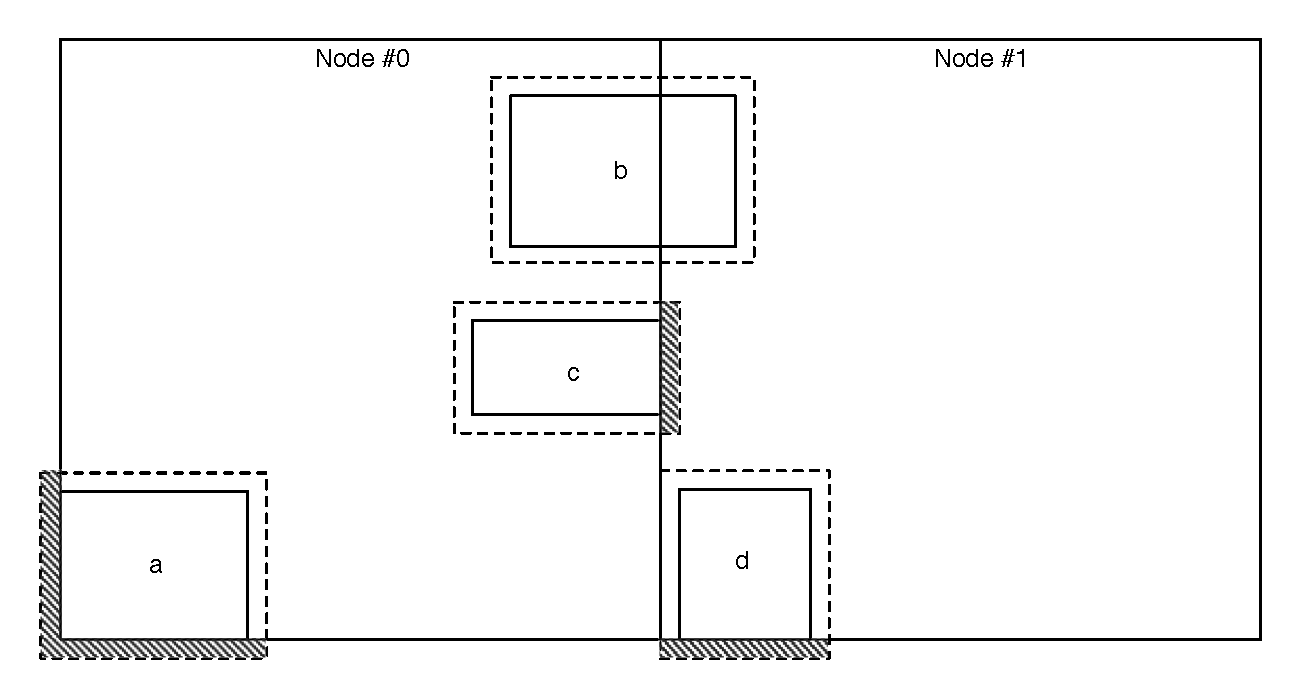
\includegraphics[width=13cm,clip]{IDsearch.eps}
\end{center}
\caption{計算領域内に存在するIDのパターンとBV情報の計算.図中のa, dのハッチング部分は計算領域外なので,BVの対象外となる.一方,cのハッチング部分は,キーIDは領域\#0内,つまり領域 \#1から見るとガイドセル上にあるが,一層拡大した領域は\#1の領域内にあるため,BVの対象となる.}
\label{fig:ID BV}
\end{figure}

\begin{figure}[htbp]
\begin{center}
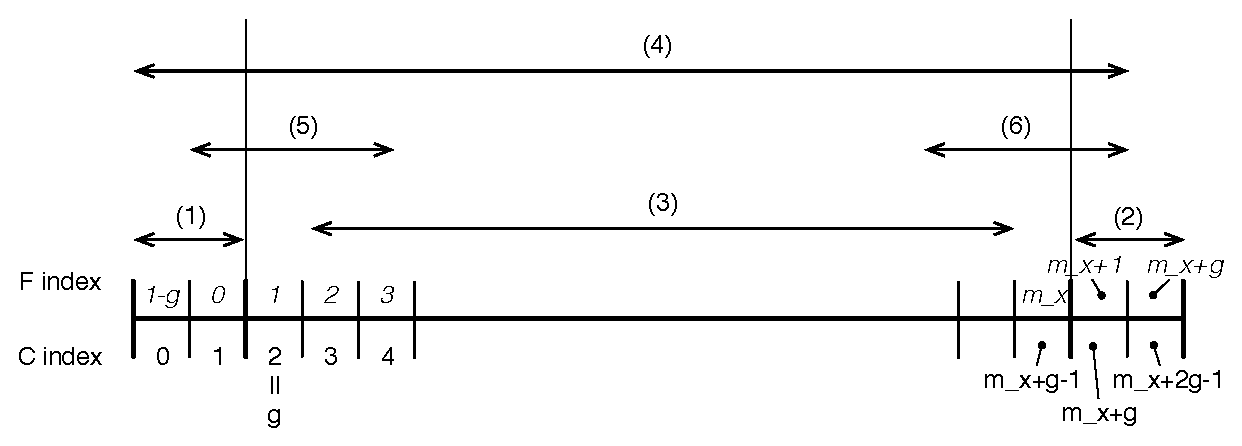
\includegraphics[width=13cm,clip]{IDpattern.eps}
\end{center}
\caption{一次元方向のIDの分布パターン.図ではガイドセル(g=2)と仮定している.処理は$(1)\sim(6)$の順番に行う.C indexからF indexへの変換は,$F_{idx} = C_{idx}+1-g$}.
\label{fig:ID pattern}
\end{figure}

一次元方向のIDのパターンを\textbf{図\ref{fig:ID pattern}}に示す.
最初に,対象IDのみが存在するBV情報は,V-Sphereのメソッド\verb|GetBndIndexExtGc()|で拡張オプションの引数0を渡して,ローカルなインデクス情報を得る.\verb|GetBndIndexExtGc()|は,各方向の開始インデクス\verb|st_i, st_j, st_k|とコンポーネントの長さ\verb|len_i, len_j, len_k|を返す.
このインデクス情報を初期値として,下記の各パターンに対して,一層拡大したインデクスを求め,所望のインデクス範囲\verb|st, ed|を得る.
以下,i方向について示す.インデクス\verb|st, ed|はFortranインデクスで保持する.
終了インデクスはCインデクスで次のように表せる.
{\small
\begin{program}
ed_i = st_i + len_i - 1;
\end{program}
}

\subsubsection{基本処理}
各ノード間のガイドセルを考慮した基本処理について示す.
以下の処理は,基本的に逐次の場合.並列時は,計算領域内か領域外かの判定が必要.
便宜的に次の変数を導入しておく.\verb|m_x|は三次元配列の各要素方向の最大値(計算内部領域)である.
{\small
\begin{program}
n_st = st_i - 1; // 一層外側へ拡大
n_ed = ed_i + 1; // 一層外側へ拡大
max_c1 = m_x + g;
\end{program}
}

また,以下のコンテキストで\verb|nID[]|には隣接6方向の各ノードのランク番号が入っており,隣接ノードがなければ負値が入っている.

\begin{description}
\item[(1)] BVがX-方向のガイドセル内のみにある場合\\
x+側に一層拡大し,その値が自領域内であれば,1層分だけ存在する.
{\small
\begin{program}
if ( ed_i < guide ) { 
  if( nID[MINUS_DIR] < 0 ){ // 計算領域の外部面に接する場合は,対象外
    m_st = 0;
    m_ed = 0;
  }
  else { // 計算領域内部にある場合(並列時)
    if ( n_ed == guide ) { // ガイドセル1層外側の場合
      m_st = 1; // F index
      m_ed = 1; // F index
    }
    else {
      m_st = 0;
      m_ed = 0;
    }
  }
}
\end{program}
}

\item[(2)] BVがX+方向のガイドセル内のみにある場合\\
x-側に一層拡大し,その値が自領域内であれば,1層分だけ存在する.
{\small
\begin{program}
if ( st_i >= max_c1 ) {
  if( nID[PLUS_DIR] < 0 ){ // 計算領域の外部面に接する場合は,対象外
    m_st = 0;
    m_ed = 0;
  }
  else {
    if ( n_st == (max_c1 - 1) ) { // ガイドセル1層外側の場合
      m_st = m_x; // F index
      m_ed = m_x; // F index
    }
    else {
      m_st = 0;
      m_ed = 0;
    }
  }
}
\end{program}
}

\item[(3)] BVが内部領域のみにある場合\\
開始点の処理は,x-側に一層拡大しその値が自領域内の端の場合,開始インデクスは領域内の最小インデクス.それ以外はマイナス1.
終点の処理は,x+側に一層拡大し,その値が自領域内の端の場合,終了インデクスは領域内の最大インデクス.それ以外はプラス1.
{\small
\begin{program}
if ( (st_i >= guide) && (ed_i < max_c1) ) {
  if ( st_i == guide ) { // 最外層セル
    m_st = 1; // F index
  }
  else {
    m_st = n_st + 1 - guide; // F index
  }
    
  if ( ed_i == (max_c1 - 1) ) { // 最外層セル
    m_ed = m_x; // F index
  }
  else { // 内部
    m_ed = n_ed + 1 - guide; // F index
  }
}
\end{program}
}

\item[(4)] BVが両方向のガイドセルにまたがる場合\\

{\small
\begin{program}
if ( (st_i < guide) && (ed_i >= max_c1) ) {
  m_st = 1; // F index
  m_ed = m_x; // F index
}
\end{program}
}

\item[(5)] BVがX-方向のガイドセルから内部領域にある場合\\
開始点は領域内の最小インデクス.終点は端点か,あるいは内部の可能性.
{\small
\begin{program}
if ( (st_i < guide) && (ed_i < max_c1) ) {
  m_st = 1; // F index
    
  if ( ed_i == (max_c1 - 1) ) { // 最外層セル
    m_ed = m_x; // F index
  }
  else { // 内部
    m_ed = n_ed + 1 - guide; // F index
  }
}
\end{program}
}

\item[(6)] BVがX+方向のガイドセルから内部領域にある場合\\
終点は領域内の最大インデクス.開始点は端点か,あるいは内部の可能性.
{\small
\begin{program}
if ( (st_i < max_c1) && (ed_i >= max_c1) ) {
  m_ed = m_x; // F index
    
  if ( st_i == guide ) { // 端点
    m_st = 1; // F index
  }
  else { // 内部
    m_st = n_st + 1 - guide; // F index
  }
}
\end{program}
}

\end{description}


上記のメソッドを各方向から利用できるように\verb|getEnlargedIndex()|を実装する.


%
\subsection{ビットフラグのエンコード処理}
BC Indexのビットフィールドへのエンコード処理を具体的に示す.

\begin{enumerate}
%
\item bcdへのエンコード(1) \verb|BinaryVoxel::setBCIndex_base1()|\\
BC Indexの配列bcd[]は,ソルバ中で共通的に利用するフラグを集めている.
ガイドセルを含む全領域に対して処理を行う.
まず,stateを流体で初期化.
次に,ボクセルモデルのセルIDを8bitでエンコードする\footnote{ID=0は使わないので,ID=1$\sim$255の範囲.}.
コンポーネントリストに登録された境界条件と媒質に対して,媒質情報にアクセスするためのMaterialList[]へのエントリをエンコードする.
最後に,各セルの媒質エントリをたどり,MaterialList[]の内容から流体か固体かを判断し,stateをエンコードする.
\vspace{2mm}

%
\item bcd[]へのエンコード(2) \verb|BinaryVoxel::setBCIndex_base2()|\\
先に設定したstateをみて,\verb|find_isolated_Fcell()|で孤立した流体セルを固体セルへ変更する.
これは,計算の不安定性を取り除くための処理で,大局的にみて影響は小さい.
この処理では,置換する固体セルは隣接固体IDの最頻値とする.

 次に,\verb|encActive()|で不活性セルの設定を行う.
不活性セルは,Kind\_of\_Solverのパラメータにより異なる処理となる.
\begin{itemize}
\item FLOW\_ONLY, THERMAL\_FLOW, THERMAL\_FLOW\_NATURAL\\
流体セルのみが計算に有効で,固体セルは不活性とする.

\item SOLID\_CONDUCTION\\
固体セルのみが計算に有効で,流体セルは不活性とする.

\item CONJUGATE\_HEAT\_TRANSFER\\
流体・固体セルともに有効.
\end{itemize}

さらに,コンポーネントで指定された不活性セルを不活性化する(Active bitをINACTIVEにする).
不活性セルの指定は,流体・固体セル両方可能.
\vspace{2mm}

%
\item bcp[]へのエンコード \verb|BinaryVoxel::setBCIndexP()|\\
bcd[]からactive, stateの両フラグをコピーし,残りのビットフラグを(1)で初期化する.
\vspace{2mm}

\begin{itemize}
\item 内部領域の処理 \verb|encPbit_Wall_Inside()|\\
内部領域にある流体セルのうち,固体セルに隣接する面のノイマンフラグ\verb|BC_N_?|をゼロにする.
外部境界面に接するセル面は後で処理.
つぎに,全内部領域について,固体セルに隣接する流体セルにwall locationフラグを付与する.
この処理は,\verb|cbc_pvec_()|などの関数で壁法則の計算に利用する.
\vspace{2mm}

\item 外部境界面の処理 \verb|BinaryVoxel::encPbit_OBC()|\\
外部境界面がDirichletかNeumannかを指定し,対応するフラグ\verb|BC_D_?|または\verb|BC_N_?|をエンコードする.
外部境界面が壁面の場合にのみ,方向フラグを付与する.
\vspace{2mm}

\item コンポーネントのエンコード\\
コンポーネントの境界条件の種類毎に処理の内容は異なる.
\begin{itemize}
\item SPEC\_VEL, SPEC\_VEL\_WH, OUTFLOW\\
テストセルが流体セルでDef\_Face IDが指定されている場合,かつ,テストセルの隣接セルが固体でキーIDの場合,テストセルの対象面にNeumannフラグをエンコードし,bcd[]にComponentList[]へのエントリを登録する.
\vspace{2mm}

\item PERIODIC, CELL\_MONITOR, IBM\_DF, HEX, FAN, DARCY\\
bcd[]にComponentList[]へのエントリを登録する処理のみ行う.
\vspace{2mm}

\end{itemize}

\item 対角・非対角要素の係数のエンコード \verb|encPbit()|\\
NeumannフラグとDirichletフラグが同時に設定されていないことを確認.
反復行列の非対角要素/対角要素をエンコードする.
対角要素がゼロの場合はエラー.
\end{itemize}
\vspace{2mm}

%
\item bcv[]へのエンコード \verb|BinaryVoxel::setBCIndexV()|\\
速度境界条件の種類をセルの各面にエンコードする.
各面に5bitを割り当てる.(0)は境界条件なし,(31)は外部境界条件,それ以外の(1$\sim$30)はコンポーネントのエントリを示す.
まず,bcd[]からactive, stateの両フラグをコピーする.

\begin{itemize}
\item 外部境界面の境界条件のエンコード \verb|BinaryVoxel::encVbit_OBC()|\\
この処理は,外部境界面に接するセルが流体の場合を対象とする.
外部境界条件の実装には,流束形式と境界値形式の2種類がある.
流束形式はOBC\_SYMMETRIC, OBC\_WALL, OBC\_SPEC\_VEL, OBC\_OUTFLOWで,境界値形式はOBC\_TRC\_FREE, OBC\_PERIODIC, OBC\_IN\_OUTである.
流束形式の場合には,セルフェイスに外部境界条件フラグ(31)をエンコードする\footnote{運動量fluxの計算で,セルフェイスが境界条件(!=0)の場合には,その流束の寄与をゼロにしておいて,後ほど境界条件による流束を加算する.}.
OBC\_SYMMETRIC, OBC\_WALLのときガイドセルが固体であることをチェックし,
OBC\_SPEC\_VEL, OBC\_OUTFLOWのとき対象セルが流体の場合のみガイドセルが流体であることをチェックする.

 境界値形式のOBC\_TRC\_FREE, OBC\_IN\_OUTの場合,対象面が流体であることのみチェックし,セルフェイスに外部境界条件フラグはエンコードしない.
つまり,通常スキームによる計算となる.
OBC\_PERIODICの場合には,外部境界条件フラグのエンコードも流体面のチェックも行わない.
\vspace{2mm}

\item 内部境界条件のコンポーネントへのエンコード \verb|BinaryVoxel::encVbit_IBC()|\\
コンポーネントがSPEC\_VEL\_WH, SPEC\_VEL, OUTFLOWの場合,キーIDは固体セル,Def\_Face IDに流体セルが指定される.
したがって,テストセルが流体でDef\_Face IDが指定され,かつ,テストセルの隣接セルが固体でキーIDの場合にのみ,エンコード処理を行う.
また,流体セルの流入出面にはコンポーネントのエントリをエンコードし,同時にbcp[]の壁面方向を表すwall locationフラグをoffにする.
これは,境界条件付与部分の固体面は,壁法則の計算を行わないようにするためである.

 内部境界条件の流入出は,ボクセルモデルでは固体セルにより流入出面が規定されている.\hyperlink{tgt:inflow}{流入出境界条件処理}で高次風上スキーム時の運動量流束の正確な計算のため,指定されたキーIDのセルを流体の状態にしておく.
\vspace{2mm}

\item セルの固体面数のエンコード \verb|encPbit_No_SolidFace()|\\
bcp[]にセルの6面のうち,固体面の数をエンコードする\footnote{粘性項の表面積補正のための実験的実装.}.
もし,6面とも固体面の場合にはエラーで停止する.

\end{itemize}

%
\vspace{2mm}

\item bch1, bch2へのエンコード \verb|BinaryVoxel::setBCIndexH()|\\
温度境界条件の情報をエンコードする.
bcd[]からactive, stateの両フラグをコピーする.
\vspace{2mm}

\begin{itemize}
\item 断熱フラグの初期化\\
bch2[]の断熱フラグを非断熱(1)に初期化する.
\vspace{2mm}

\item Kind\_of\_Solverのパラメータに応じて,Solid-Fluid面の断熱処理\\
THERMAL\_FLOW, THERMAL\_FLOW\_NATURALの場合,FluidセルのうちSolidセルに接する面について,\verb|setAmask_Thermal()|でbch2[]の断熱フラグを断熱(0)にする.
SOLID\_CONDUCTIONの場合,SolidセルのうちFluidセルに接する面について,\verb|setAmask_Solid()|でbch2[]の断熱フラグを断熱(0)にする.
\vspace{2mm}

\item 対称境界面に断熱マスクをセット\\
対称境界が指定された外部境界面に対して,\verb|encAmask_SymtrcBC()|でbch2[]の断熱フラグを断熱(0)にする.
\vspace{2mm}

\item 不活性セルの場合の断熱マスク処理\\
コンポーネントで指定された不活性セルIDに対して,\verb|setAmask_InActive()|でセルをInactiveにする.
流体セル,固体セルに関わらず,隣接セルがInactive指定の場合には断熱にするが,自セルが指定ID以外のときに限る.
つまり,Inactiveに指定したセルと接するセルの隣接面を断熱にする.ただし,隣接セルは非Inactive指定であること.
これは,Inactive指定セルが塊の時には,その内部はラプラスを解き,平均場にするため.
\vspace{2mm}

\item コンポーネントのエンコード\\
各コンポーネント毎の処理を行う.
\vspace{2mm}

\begin{description}
\item[-] 断熱条件 \verb|encQface()|\\
テストセルがDef\_Faceで,隣接セルがキーIDのセルで挟まれる面に対して,bch1[]にCompoListのエントリをエンコードし,
bch2[]に断熱条件(0)をエンコード.
\vspace{2mm}

\item[-] 熱流束指定 \verb|encQface()|\\
テストセルがDef\_Faceで,隣接セルがキーIDのセルで挟まれる面に対して,bch1[]にCompoListのエントリをエンコードし,
bch2[]に非断熱条件(1)をエンコード.
\vspace{2mm}

\item[-] 流入・流出指定 \verb|encQfaceSVO()|\\
コンポーネントがSPEC\_VEL\_WH, OUTFLOWの場合,キーIDは固体セル,Def\_Face IDに流体セルが指定される.
テストセルがDef\_Face IDで指定され,かつ,隣接セルがキーIDの場合にのみ,
bch1[]にCompoListのエントリをエンコードし,bch2[]に非断熱条件(1)をエンコードする.\verb|BinaryVoxel::encVbit_IBC()|の場合とは異なり,セルの状態をチェックしない.
\hyperlink{tgt:inflow}{流入出境界条件処理}で高次風上スキーム時の対流熱流束の正確な計算のため,指定されたキーIDのセルを流体の状態にしておく.
\vspace{2mm}

\item[-] 熱伝達指定 Type\_S \verb|encQfaceHT_S()|\\
Kind\_of\_SolverがTHERMAL\_FLOWまたはTHERMAL\_FLOW\_NATURALの場合に,コンポーネントHeatTransfer\_S, HeatTransfer\_SN,HeatTransfer\_SFを指定できる.
キーIDは固体セル,Def\_Face IDに流体セルが指定される.
テストセルがDef\_Face IDかつ流体で指定され,かつ,隣接セルがキーIDかつ固体の場合にのみ,
bch1[]にCompoListのエントリをエンコードし,bch2[]に非断熱条件(1)をエンコードする.
\vspace{2mm}

\item[-] 熱伝達指定 Type\_B \verb|encQfaceHT_B()|\\
Kind\_of\_SolverがCONJUGATE\_HEAT\_TRANSFERまたはSOLID\_CONDUCTIONの場合に,コンポーネントHeatTransfer\_Bを指定できる.
キーIDは固体セル,Def\_Face IDに流体セルが指定される.
テストセルがキーIDかつ固体で指定され,かつ,隣接セルがDef\_Faceかつ流体の場合にのみ,
bch1[]にCompoListのエントリをエンコードし,bch2[]に非断熱条件(1)をエンコードする.
\vspace{2mm}

\item[-] 等温指定 \verb|encQfaceISO_SF/SS()|\\
等温境界条件は,流体と固体,あるいは固体と固体で挟まれる面に対して適用可能である.
流体と固体セルの間で指定される等温境界は,Kind\_of\_SolverがTHERMAL\_FLOWまたはTHERMAL\_FLOW\_NATURALの場合に用いられる.
このとき,キーIDに固体セル,Def\_Face IDには流体セルが指定される.
テストセルがDef\_Face IDかつ流体で指定され,かつ,隣接セルがキーIDかつ固体の場合に,bch1[]にCompoListのエントリをエンコードし,bch2[]に非断熱条件(1)をエンコードする.

 一方,固体セル間の面で指定される等温境界は,Kind\_of\_SolverがCONJUGATE\_HEAT\_TRANSFERまたはSOLID\_CONDUCTIONの場合に用いられる.
このとき,キーIDセルとDef\_Face IDセルは両方とも固体セルである.
テストセルがキーIDかつ固体で,Def\_Face ID(固体セル)と挟まれる面に対して,bch1[]にCompoListのエントリをエンコードし,bch2[]に非断熱条件(1)をエンコードする.
\vspace{2mm}

\item[-] 熱源指定\\
熱源のタイプとして,Heat\_SourceとConstant\_Temperatureの2種類の指定方法がある.
これらの境界条件は,体積要素に対する指定である.
テストセルが指定されるIDの場合,bch2[]にCompoListのエントリをエンコードする.

\end{description}

\vspace{2mm}

\item 熱境界フラグの設定 \verb|encHbit()|\\
GMA\_?のフラグをセットする.まず,(1)で初期化.
bch1[]の各セルフェイスフラグBC\_FACE\_?をみて,境界条件があればbch2[]のGMA\_?を(0)にする.
その後,対角要素の係数を断熱マスクを考慮して計算し,H\_DIAGに対角要素の係数(0$\sim6$)をストアする.
もし,対角要素が(0)であればゼロ割防止のために(1)を入れておく.対角要素がゼロのセルは境界条件や断熱セルで囲まれたセルに相当する.
\end{itemize}


%
\vspace{2mm}

\end{enumerate}





BC Index bx[] は図\ref{fig:Decode}を参照して下記のコードのように利用する.この例では速度の境界条件について説明している.まず,setInnerVBCface()で境界条件のループnを回し,それがフェイス面に対する速度境界条件であれば(isVBCF()),処理を行う.次に,cmp[n].getType()の値により,n番目に登録された境界条件の種類を特定する.その後,個別の処理を行う.setDirichletVInside()では,指定された面に速度成分を与える処理を行っている.空間ループを回し,bx[i,j,k] の値がエンコードされた境界条件の格納番号,および方向と一致する場合に目的の処理を行う.このとき,必要に応じて MaterialListに登録された物性値を利用する.

{
\small
\begin{verbatim}
/**
 @fn void SetBC3D::setInnerVBCface(SKL_REAL* v, unsigned* bx, SKL_REAL v00, ...)
 @brief 速度の内部境界をセットする
 @param v 速度ベクトル
 @param bx BCindex
 @param v00 基準速度情報
 @param tm 時刻
 @param arrangement 格子配置
 */
void SetBC3D::setInnerVBCface(SKL_REAL* v, unsigned* bx, SKL_REAL v00, 
                                      SKL_REAL tm, const char* arrangement)
{
  for (unsigned n=1; n<=NoBC; n++) {
    if ( cmp[n].isVBCF() ) {

      switch ( cmp[n].getType() ) {
        case DIRICHLET_INSIDE:
				case DIRICHLET_CTMP:
          if ( !strcasecmp("staggered", arrangement)) {
            if ( cmp[n].usw != DRC_V_SHO ) {
                  cmp[n].val[0] = setDirichletV_Inside_S(v, bx, n, v00);
            }
            else {
                  cmp[n].val[0] = setSHO_Inside_S(v, bx, n, tm, v00);
            }
          }
          else if ( !strcasecmp("collocated", arrangement)) {
            ;
          }
          else {
            stmpd_printf("Invalid keyword\n");
          }
          break;
          
        default:
          break;
      }

    }
  }
}

/**
 @fn SKL_REAL SetBC3D::setDirichletVInside(SKL_REAL* v, unsigned* bx, unsigned n, SKL_REAL v00)
 @brief 内部領域の速度のディリクレ境界をセットする
 @param v 速度ベクトル
 @param bx BCindex
 @param n 境界条件コンポーネントのエントリ番号
 @param v00 参照速度
 @retval 無次元平均流速
 @note
    - 内部境界はセル面直を仮定
 */
SKL_REAL SetBC3D::setDirichletV_Inside_S(SKL_REAL* v, unsigned* bx, unsigned n, SKL_REAL v00)
{
  unsigned i, j, k, s;
  SKL_REAL va=0.0;
  SKL_REAL vel, vec[3];
  
  vel   = cmp[n].N1.Velocity * v00;
  
  vec[0]= cmp[n].nv[0]*vel;
  vec[1]= cmp[n].nv[1]*vel;
  vec[2]= cmp[n].nv[2]*vel;
  
  for (k=cmp[n].ci.st[2]; k<=cmp[n].ci.ed[2]; k++) {
    for (j=cmp[n].ci.st[1]; j<=cmp[n].ci.ed[1]; j++) {
      for (i=cmp[n].ci.st[0]; i<=cmp[n].ci.ed[0]; i++) {
        s = bx[ SklUtil::getFindexS3D(size, guide, i, j, k) ];
        if ( FBUtility::chkBCOrder(s, n) ) {
          if ( FBUtility::chkShift(s, VFACE_I) ) {
            va += v[SklUtil::getFindexV3D(size, guide, i, j, k, 0)] = vec[0];
          }
          if ( FBUtility::chkShift(s, VFACE_J) ) {
            va += v[SklUtil::getFindexV3D(size, guide, i, j, k, 1)] = vec[1];
          }
          if ( FBUtility::chkShift(s, VFACE_K) ) {
            va += v[SklUtil::getFindexV3D(size, guide, i, j, k, 2)] = vec[2];
          }
        }
      }
    }
  }
  va = va * dh*dh / (SKL_REAL)cmp[n].area;
  return (va);
}
\end{verbatim}
}

\begin{figure}[htbp]
\begin{center}
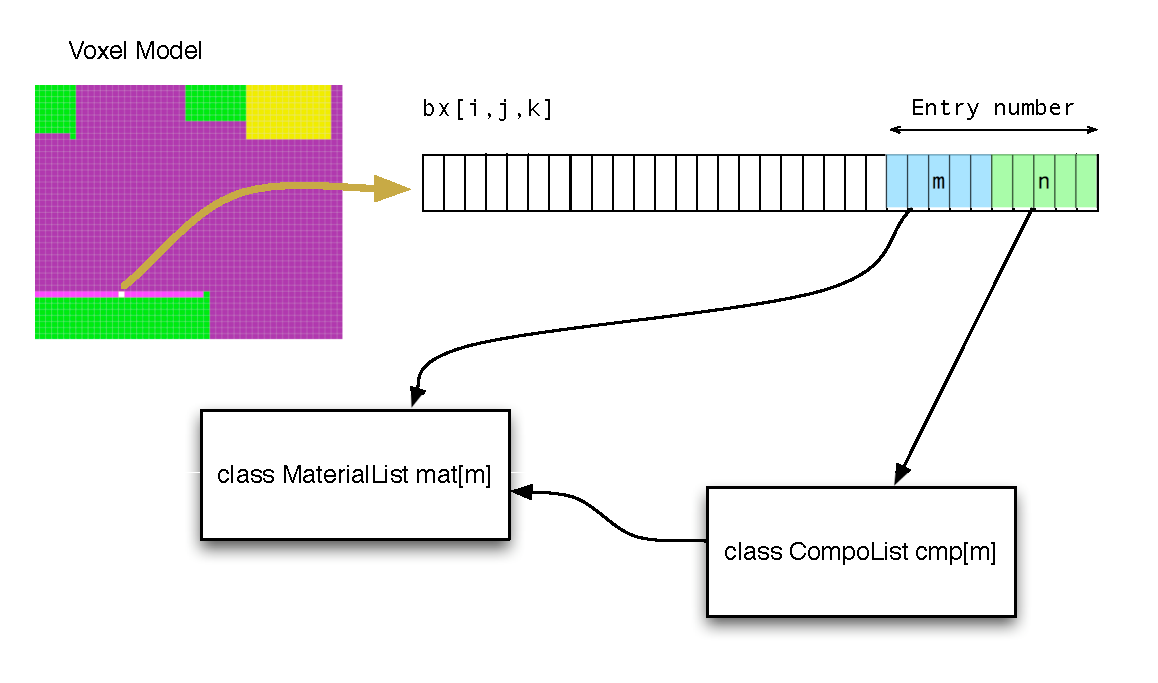
\includegraphics[width=12cm,clip]{Decode.eps}
\end{center}
\caption{BC Indexからのビットフラグのデコード}
\label{fig:Decode}
\end{figure}


%
\subsection{セルフェイスに対する速度境界条件}
スタガード変数配置における各速度成分に対して値を指定する.例として,図\ref{fig:cell face BC}に示すようなバイナリボクセルモデルにおいて,矢印方向の速度成分を与えることを考える.IDとして,空間に1, 3が指定されている.このとき,矢印の方向ベクトルは(0,1,0)でID=3とID=1が接する面であるので,以下のようなXMLで大きさ0.58の一定な速度成分を指定する.

\begin{figure}[htbp]
\begin{center}
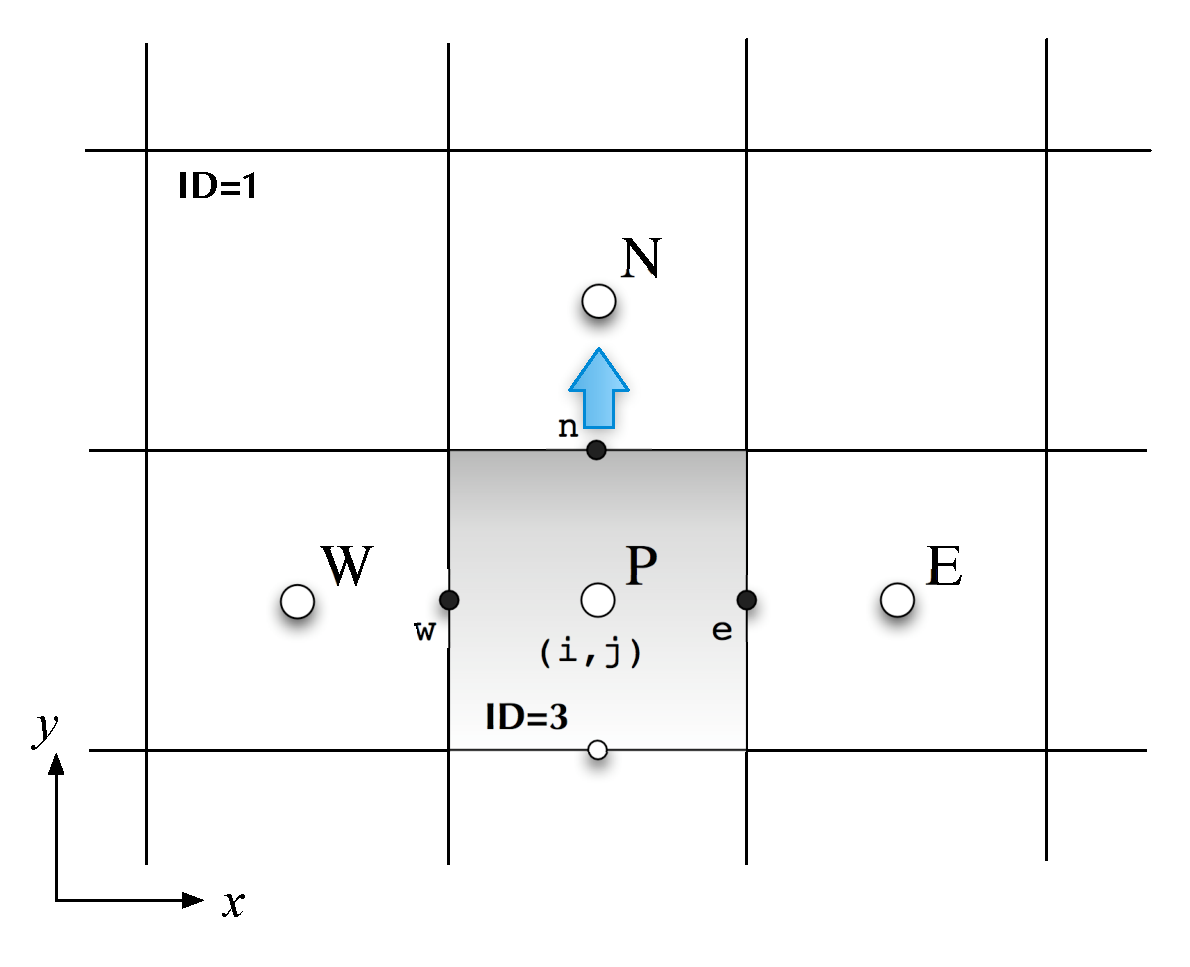
\includegraphics[width=8cm,clip]{Vface-mid.eps}
\end{center}
\caption{セルフェイスにおける速度境界条件}
\label{fig:cell face BC}
\end{figure}

{
\small
\begin{verbatim}
<InnerBoundary>
  <Elem name="Vec_Face" id="1">
    <Elem name="Dirichlet" id="3" comment="source">
      <Param name="Norm_x"      dtype="REAL"   value="0.0" />
      <Param name="Norm_y"      dtype="REAL"   value="1.0" />
      <Param name="Norm_z"      dtype="REAL"   value="0.0" />
      <Param name="velocity"    dtype="REAL"   value="0.58" />
      <Param name="def_face"    dtype="INT"    value="1" />
      <param name="type"        dtype="string" value="constant" />
    </Elem>
  </Elem>
</InnerBoundary>
\end{verbatim}
}

%
\subsection{セルフェイスに対する熱境界条件}
\begin{indentation}{3zw}{0zw}
{
熱境界条件をコンポーネントとして与える場合,基本的に,固体面に与える.
\textbf{図\ref{fig:heat bc on solid}}に示すように,固体面から流体側へ法線を考えて,法線方向が指定値の正の値とする.
つまり,流体側への熱移動が正の方向となるように考える.

\begin{figure}[htbp]
\begin{center}
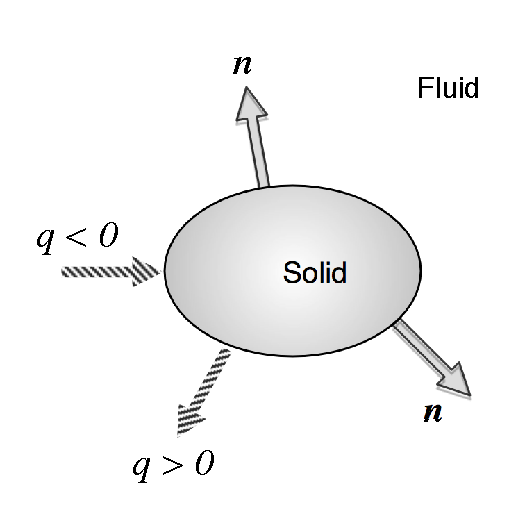
\includegraphics[width=6cm,clip]{heatBC.eps}
\end{center}
\caption{流体-固体界面における熱境界条件の指定方法}
\label{fig:heat bc on solid}
\end{figure}

この考え方に基づくと,Solver\_PropertyのKind\_of\_Solverの指定モードによって,熱境界条件の働きが異なる.
Thermal\_FlowとThermal\_Flow\_Naturalの場合は,熱流動計算で流体の温度のみが意味を持ち,固体部分は計算対象とはならず不活性セルとして扱う.
したがって,流体-固体の境界面で与える熱境界条件(熱流束)は,流体セル側のみに指定する.

一方,Solid\_Conductionの場合は固体部分の熱伝導のみを解くので,流体部分は不活性セルとして扱う.
したがって,流体-固体の境界面で与える熱境界条件は,固体セル側のみに指定する.

また,Conjugate\_Heat\_Transferの場合には流体と固体の熱移動を計算する.
したがって,流体-固体の境界面で与える熱境界条件は,流体セルと固体セルの両方で指定する.

以下の各境界指定で述べるように,IDとDef\_Faceタグの組み合わせにより,流体-固体の境界面を指定する.
このとき,IDには固体のIDを,Def\_Faceには流体または固体のIDを指定することを基本とする\footnote{IDに固体を指定する理由は,固体面は大抵の場合局所的なので,参照範囲を小さく抑えて効率的な計算をするため.}.


境界条件の処理手順は次のとおり.
\begin{enumerate}
\item \verb|SetBC3D::InnerTBCface()|\\
拡散項に関するセルフェイスの熱境界条件処理.
コンポーネントのループを回し,対象境界条件を特定し,各処理に分岐.
熱流束指定の場合には\verb|SetBC3D::ps_IBC_Heatflux()|で境界条件を計算.
戻り値をコンポーネントのモニタ保持変数に代入.
\vspace{2mm}

\item \verb|SetBC3D::ps_IBC_Heatflux()|\\
与える熱流束を有次元から無次元に変換.
各コンポーネントリストのBVループ範囲のセルに対して,セルを構成する各面に境界条件が指定されているかどうかをテストする.
対象となる面に対しては,熱流束を保持する配列\verb|qbc|に値をストアする.
スタガードのインデクスに注意.
セルのW面における正値$(q \ge 0)$は流入で,E面における正値$(q \ge 0)$は流出となる.
この関数内でallreduce()をかけ,無次元熱流束を集約,返値にする.
\end{enumerate}


上記の処理を行うための前処理として,次の処理を行っておく.
\begin{enumerate}
\item \verb|BinaryVoxel::setBCIndexH()|\\
熱境界条件のビットインデクスをエンコードする.
\begin{itemize}
\item まず,セルの各面の断熱マスク(6面分)を非断熱(1)に初期化する.
\item モードに応じて,流体-固体界面を断熱(0)にする.
\begin{description}
\item[-] THERMAL\_FLOWとTHERMAL\_FLOW\_NATURALの場合,\verb|BinaryVoxel::setAmask_Thermal()|で,S-F面のF側を断熱にする.
\item[-] SOLID\_CONDUCTIONの場合は,\verb|BinaryVoxel::setAmask_Solid()|で,S-F面のS側を断熱にする.
\item[-] CONJUGATE\_HEAT\_TRANSFERの場合には,固体セルも流体セルも両方とも計算するので,断熱処理はしない.
\end{description}

\item 対称境界面に断熱マスクをセット\\
\item 不活性セルの場合の断熱マスク処理\\
\item 媒質コンポーネントに対して,elementをセット\\
\item 具体的なエンコード処理\\
\item 係数行列の値をビットでエンコード\\
\verb|BinaryVoxel::encHbit()|で,\verb|bh2[]|の$\gamma$を1で初期化.
\verb|bh1[]|を調べて,セルの各面に境界条件がセットされていなければ(!=0),\verb|bh2[]|の各面で$\gamma=1$とする.
対角要素の係数は$\sum \limits_j=0^5 \left( \gamma_{BC} \gamma_A \right)_j$として,断熱マスクを考慮.
\end{itemize}



\vspace{2mm}

\item 
\end{enumerate}



\vspace{20mm}

ボクセルモデルのセルフェイスに対する熱境界条件 QBC\_Face の具体的な種類は,XMLファイルに記述された内容を基にしてCompoList クラスのオブジェクトのメンバー変数,compo[n].type にエンコードする.

図\ref{fig:BCIndex}のBC Index の$17\sim22$ビットにおいて,セルの6面に対して BC の種類を判別するフラグを持たせるのは,隣接セルとの重複があるため冗長であるが,BC Index の値をロードした後ビット演算だけで済む.よって,メモリアクセスが少ないので効率が良い.
セル P の全てのプラス方向の面に対してエンコード処理を行い,その後プラス方向の面の情報を隣のセルのマイナス方向にコピーする.

BCフラグの値は,下記の疑似コードのように利用する.
{
\small
\begin{verbatim}
/**
 @fn void FBUtility::getBCgamma (unsigned idx, SKL_REAL* a)
 @brief γの値から係数を配列で返す
 @retval γ
 @param idx BCindex
 @param a 係数配列
 */
void FBUtility::getBCgamma(unsigned idx, SKL_REAL* a) 
{
  a[0] =(SKL_REAL)( (idx >> GMA_W) & 0x1 );
  a[1] =(SKL_REAL)( (idx >> GMA_E) & 0x1 );
  a[2] =(SKL_REAL)( (idx >> GMA_S) & 0x1 );
  a[3] =(SKL_REAL)( (idx >> GMA_N) & 0x1 );
  a[4] =(SKL_REAL)( (idx >> GMA_B) & 0x1 );
  a[5] =(SKL_REAL)( (idx >> GMA_T) & 0x1 );
}
\end{verbatim}
}
QBC\_Face の具体的な境界条件は,前述のXMLファイルに記述された内容を基に判断する.
次節以降で具体的な境界条件について述べる.
}
\end{indentation}







%
\subsection{外力を用いた境界条件の実装}
\label{sec:implementation external force}
\ref{sec:external force method}で説明した外力項による境界条件について,その実装を説明する.



%
\subsection{Immersed Boundaryを用いた境界条件の実装}
\label{sec:implementation of IB}

\ref{sec:Immersed Boundary Method}で述べたImmersed Boundary Methodの実装について説明する.計算する格子系としては,StaggeredとCollocatedの2種類がある.そのため,前処理では格子配置に応じて内部処理が異なる.図\ref{fig:IBmask}に示すように,変数配置により指定したセル領域内にかかる速度定義点が異なる.このため,Staggeredではセル境界に与える境界条件VBCFで記述し,Collocatedではセルセンターに与える境界条件VBCCで記述する.
Staggeredの場合には,セルに与えられたDirect\_ForcingのIDを見つけると,そのセルの両端にあるセル界面位置の速度定義点をForcingの対象とする.これに対して,Collocatedの場合には,セルセンターの速度定義点のみがForcingの対象となる.

解法で述べたように,Direct Forcingは速度の強制で実装するので,内部的にはディリクレ型速度境界条件を使って実装する.
また,Direct Forcingは流体セルに対して有効であるので,Active\_BitはONにしておく.

\begin{figure}[htbp]
\begin{center}
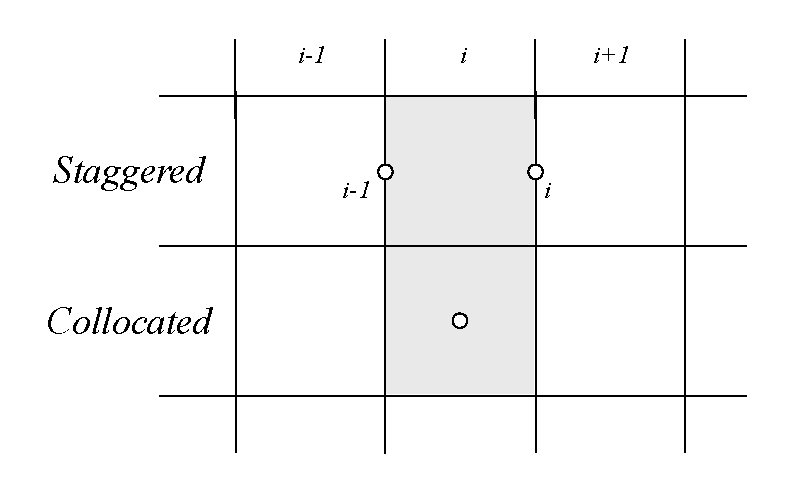
\includegraphics[width=8cm,clip]{IB_mask.eps}
\caption{Direct Forcningのセル指定と強制対象となる速度位置の関係}
\label{fig:IBmask}
\end{center}
\end{figure}


%
\subsection{V-Sphereコンポーネントを用いた実装}
全計算領域の一部に存在する内部境界条件要素(コンポーネント)の実装にV-Sphereにより提供されるComponent機能を用いる.この機能には,並列処理時のサブドメイン間のデータ通信や管理が含まれ,均等分割とマルチボックス分割の両方に対応する.

\begin{enumerate}
\item 全計算領域のボクセル情報の初期化\\ 
\verb|SklSolverC3D::VoxelInitialize()|
\item Bounding Boxのグローバル情報の取得\\ 
\verb|SklSolverC3D::getGlobalCmpIdx_SubVoxInit()|
\item コンポーネント領域の初期化と登録\\ 
\verb|SklSolverC3D::getGlobalCmpIdx_SubVoxInit()|
\item コンポーネントへのデータクラスの追加\\ 
\verb|SklSolverC3D::allocArray_forcing (long &total, int para_key)|\\
dc\_bsi(スカラ), dc\_cfr(ベクトル)のデータクラスをコンポーネントでインスタンスする.
\item コンポーネントの存在するセルに体積率を与える\\
\verb|BinaryVoxel::setCmpFractionBV()|
dc\_cfrに体積率を保持する.
\end{enumerate}



%
\section{境界条件}
境界条件の本体は主にFortran90で記述している.Fortran コードは,C++の名前空間内ではCソースコードと同様に名前なし空間として扱われるので,FortranFuncC3D.h内にプロトタイプを記述しておく.

\subsection{外部境界条件の実装}
外部境界条件は,計算領域の外周に設定する境界条件である.
各節で,速度,圧力,温度に対する境界条件を説明する.
Fortranコードは,SetBC3Dクラスに実装されたメソッドsetOuterPBC, SetOuterTBC, setOuterVBC内でハンドリングされている.
Fortranコードには,たとえば流出境界条件ならば,計算領域の$X\pm$面,$Y\pm$面,$Z\pm$面の各面に対する処理が書かれている.
このサブルーチンをコールするときに,方向と必要なパラメータをセットすることで必要な面の境界条件を設定する.

\begin{verbatim}
#define X_MINUS 0
#define X_PLUS  1
#define Y_MINUS 2
#define Y_PLUS  3
#define Z_MINUS 4
#define Z_PLUS  5
\end{verbatim}



%
\section{温度輸送方程式の実装}
\subsection{Euler陽解法}
式(\ref{eq:pscalar ee2})を$\Delta$形式にして解く.

\begin{equation}
\theta^{n+1} \,=\, \theta^{n} \,+\, \Delta \theta^{n+1}
\label{eq:delta form 1}
\end{equation}

\begin{equation}
\Delta \theta^{n+1} \,=\, \Delta t \, f \left( u_{i}, \, \theta \right)
\label{eq:delta form 2}
\end{equation}

式(\ref{eq:delta form 2})の$f \left( u_{i}, \, \theta \right)$は式(\ref{eq:pscalar ee2})の右辺である.
\verb|SklSolverCBC::PS_E_CBS()|メソッド内では,次のように実装している.

\begin{enumerate}
\item 対流熱流束の計算\\
\verb|cbc_tfx_cnv_uwd_()|または\verb|cbc_tfx_cnv_muscl_()|で対流熱流束を求める.流入境界条件を指定している場合には,計算した対流熱流束に上書きする形で与えている.
\item 対流項の増分\\
ConvectionEE()で対流項の増分を計算する.
\item 境界条件\\

\end{enumerate}




